\section*{応用問題1}\label{ux5fdcux7528ux554fux984c1}
\addcontentsline{toc}{section}{応用問題1}

\subsection*{(1)}\label{section}
\addcontentsline{toc}{subsection}{(1)}

最尤推定を用いて各都市ごとの回帰直線を求めると、次のような結果が得られた。

\begin{figure}
\centering
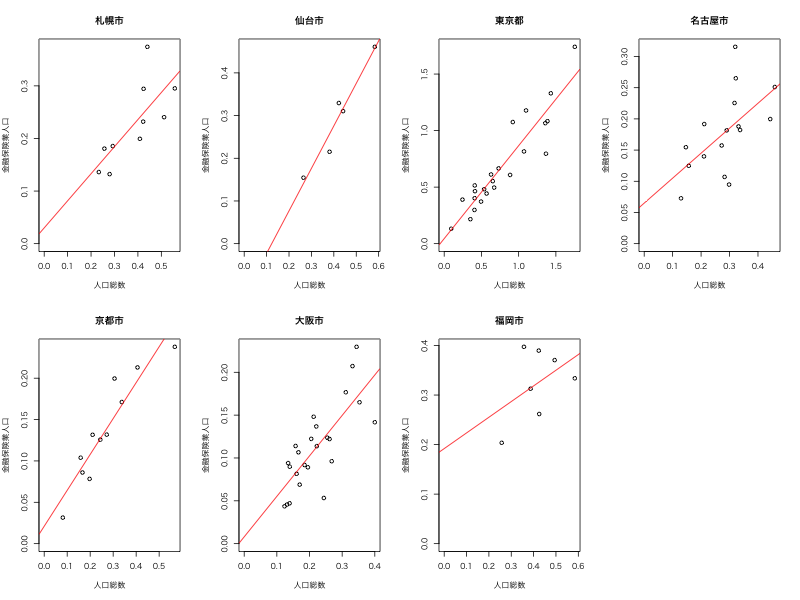
\includegraphics[width=14.00000cm]{../src/output/image/regression.png}
\caption{最尤推定法による推定}
\end{figure}

\subsection*{(2)}\label{section-1}
\addcontentsline{toc}{subsection}{(2)}

階層ベイズ法を適用する際、StanというMCMCサンプラーを用いて推定した。

データから\(\sigma_Y\)、\(a\)、\(b\)、\(\sigma_a\)、\(\sigma_b\)を推定する。
\(Y\) は各年ごとのパラメータである。\(a\), \(b\) の平均を \(\hat{a}\),
\(\hat{b}\), \(\sigma_a\) と \(\sigma_b\) は \(a\) と \(b\)
を決めるハイパーパラメータとする。また、 \(PRE[n]\)
は各都市における値である。 Stanで書いたモデルのモデル式は次の通り。

\[
Y[n] \sim Normal(b[PRE[n]] + a[PRE[n]] \times X[n], \sigma_Y)
\] \[
a[k] \sim Normal(\hat{a}, \sigma_a)
\] \[
b[k] \sim Normal(\hat{b}, \sigma_b)
\]

この書き方は、「すべての都市の平均を \(\hat{a}\), であり、各都市の
\(a[k]\) は \(\hat{a}\)
を平均とした正規分布から生成された」という書き方になっている。\(\hat{b}\)
と \(b[k]\) についても同様である。

推定の結果は次のようになった。

\begin{figure}
\centering
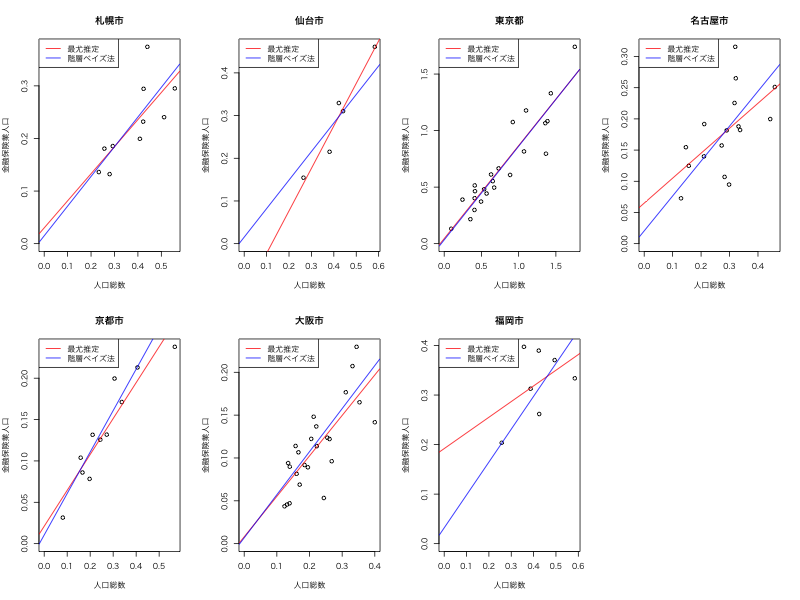
\includegraphics[width=14.00000cm]{../src/output/image/mle-mcmc.png}
\caption{階層ベイズ法と最尤推定法の比較}
\end{figure}

\subsection*{(3)}\label{section-2}
\addcontentsline{toc}{subsection}{(3)}

最も推定が大きく異なる都市は \textbf{福岡市}
である。考えられる原因は以下の通り、

\begin{enumerate}
\def\labelenumi{\arabic{enumi}.}
\tightlist
\item
  サンプル数が他の年に比べて少なく、ランダムネスによる影響が大きいため。
\item
  サンプルが少ない上に、点同士が反発しているような配置になっているため、よりランダムネスの影響を受けやすい(名古屋市も反発しているような配置になっているが、サンプル数が福岡市より多いため、最尤推定法と階層ベイズ法の差が福岡市に比べ小さいことより)。
\end{enumerate}

また、もっとも \(a(k)\) が大きい都市 \(k\) は \textbf{東京都} である。

\section*{応用問題2}\label{ux5fdcux7528ux554fux984c2}
\addcontentsline{toc}{section}{応用問題2}
